\documentclass[11pt,a4paper]{article}
\usepackage[latin1]{inputenc}
\usepackage[margin=1in]{geometry}
\usepackage{amsmath}
\usepackage{amsfonts}
\usepackage{amssymb}
\usepackage{graphicx}
\usepackage{enumitem}
\usepackage{listings}
\usepackage{color}

\definecolor{dkgreen}{rgb}{0,0.6,0}
\definecolor{gray}{rgb}{0.5,0.5,0.5}
\definecolor{mauve}{rgb}{0.58,0,0.82}

\lstset{frame=tb,
 language=MatLab,
 aboveskip=3mm,
 belowskip=3mm,
 showstringspaces=false,
 columns=flexible,
 basicstyle={\small\ttfamily},
 numbers=none,
 numberstyle=\tiny\color{gray},
 keywordstyle=\color{blue},
 commentstyle=\color{dkgreen},
 stringstyle=\color{mauve},
 breaklines=true,
 breakatwhitespace=true,
 tabsize=3
}

\setlength\abovedisplayskip{0pt}
\author{James Brissette}
\title{CS-6210: HW 3}
\begin{document}
	\maketitle
	
	\section{Chapter 5}
		\begin{itemize}
			\item[5.10]
				\begin{enumerate} [label={\alph*)}]
					\item ~
					\begin{lstlisting} 
					\end{lstlisting}
					\item ~
					
					\item ~
					\item ~
				\end{enumerate}
					
			\item[5.11]
				\begin{enumerate} [label={\alph*)}]
					\item For $g(x)$ to be a cubic spline, the following basic conditions must be met:
					$$\begin{array}{cc}
						g_1(x_1)=y1 & g_1(x_2)=y2 \\
						g_2(x_2)=y2 & g_2(x_3)=y3 
					\end{array}$$~
					$$\begin{array}{c}
						g'_1(x_2)=g'_2(x_2)\\
						g''_1(x_2)=g''_2(x_2)
					\end{array}$$
					In an attempt to find the relationship between $\alpha$ and $\beta$, and in order to deduce the values that make $g'_1(x_2)=g'_2(x_2)$ true, we equate the derivatives of $g_1$ and $g_2$ and we see that @ $x=0$ this is true for all values of $\alpha$ and $\beta$:
					$$6x+3\alpha x^2=2 \beta x + 3x^2 \rightarrow \quad true \quad \forall \alpha,\beta \quad @x=0$$
					Taking the second derivatives we see that for $6+6\alpha x = 2 \beta + 6x$ that at the point where the two curves meet ($x=0$), we get $2\beta = 6$ or $\beta = 3$. Again here we see that the we're not constrained to a specific value of $\alpha$. As an aside, interestingly enough if you plug $\beta = 3$ back into the first derivatives and set them equal to each as we did before, you find that $\alpha = -1$ for every value of x where $x\neq0$ and plugging that $\alpha$ and $\beta$ into $g_1$ and $g_2$ you see that they're equivalent for all values of x:
					$$g_1 = 2+3x^2 -x^3 \quad @\alpha=-1$$
					$$g_2 = 2+3x^2 -x^3 \quad @\beta=3$$
					
					\item Taking $\beta = 3$ we have points $(1,4)$,$(0,2)$ and if we assume $\alpha=-1$, (-1,6). If we don't make that assumption, we have $(-1,5-\alpha)$
					\item We can find the value for which $g(x)$ is a natural cubic spline by setting the second derivatives of $g_1$ and $g_2$ at the endpoints to 0 and solving for $\alpha$ and $\beta$:
					$$\begin{array}{ccc}
					s_1''(-1) = 0 & & s_2''(+1) = 0 \\
					6+6\alpha x = 0 & & 2\beta - 6x = 0 \\
					6\alpha=6 & & \beta = 3 \\
					\alpha=1 & &
					\end{array}$$
					\item We can find the value for which $g(x)$ is a clamped cubic spline by setting the first derivatives of $g_1$ and $g_2$ equal to $y'$ at the endpoints and solving for $\alpha$ and $\beta$. However, since we don't have a distinct value for $\alpha$ from part a, we can't find an exact solution:
					$$\begin{array}{ccccc}
					s_1'(-1) & = & 6x + 3\alpha x^2& = & y'_{-1} \\
					s_1'(-1) & = & -6 + 3\alpha & = & y'_{-1} \\
					 & & \alpha & = & (y'_{-1} + 6)/3 \\
					  & & & & \\
					s_2'(1) & = & 2 \beta x - 3 x^2& = & y'_{+1} \\
					s_2'(1) & = & 2 \beta- 3 & = & y'_{+1} \\
					& & 3 & = & y'_{+1}
					\end{array}$$
				\end{enumerate}
				
			\item[5.15]
				\begin{enumerate} [label={\alph*)}]
					\item Fitting the data with a global polynomial using Lagrange interpolation, and a natural cubic spline:
					\begin{center}
						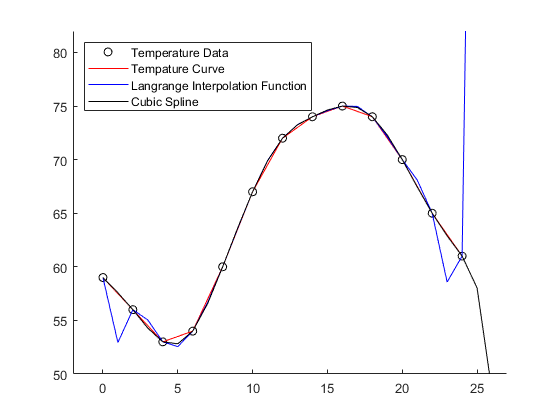
\includegraphics[width=1\linewidth]{ch5q15}
					\end{center}
				The code was all self-written and is located at the end of this file.\\
				
					\item At 11 AM the two interpolation functions give the following:
					$$\begin{array}{ccc} 
					Lagrange & & Natural Cubic Spline \\
					6.9913129e+01 & & 6.9881177e+01 \\
					69.9^{\circ} & & 69.8^{\circ}
					\end{array} $$
					\item At 1 AM the next day the two interpolation functions give the following:
					$$\begin{array}{ccc} 
					Lagrange & & Natural Cubic Spline \\
					1.5204891e+02 & & 5.8029609e+01 \\
					152.05^{\circ} & & 58.03^{\circ}
					\end{array} $$
					\item At 9 AM the next day the sun hides it face for shame at the blazing temperature Lagrange has unleashed upon the world:
					$$\begin{array}{ccc} 
					Lagrange & & Natural Cubic Spline \\
					4.5226229e+05 & & 0 \\
					452,262.29^{\circ} & & 0^{\circ}
					\end{array} $$
					Fun fact, this is about 1.8x hotter than the dead star at the center of the Red Spider Nebula $(\approx 250,000^{\circ})$ which itself is 25 times hotter than the surface of the sun.
				\end{enumerate}
				
			\item[5.22]
				\begin{enumerate} [label={\alph*)}]
					\item Looking first at Lagrange interpolation, we know that the polynomial $p_n(x)$ is a summation as follows:
					$$p_n(x) = \Sigma_{i=1}^{n+1} yi\ell_i(x), \quad where \quad \ell_i= \prod_{j=1,i \neq j}^{n+1} \frac{x-x_j}{x_i - x_j}$$
					In the formation of the Lagrange coefficient we see two subtractions and one division (3 FLOPS), which are done $n$ times ($n+1$ - 1 (when $i=j$)). The calculated coefficient is then multiplied by the value $y_i$ (add 1) $n+1$ times (multiply by $n+1$). From this we have $(3n+1)(n+1)$. Lastly, each of the those terms is the summed, for a total of $n$ additions. This gives us $(3n^2+3n+n+1)+(n) = 3n^2+5n+1$. \\
					
					Looking next at the piecewise linear interpolation, we have:
					$$G_i(x) = G(\frac{x-x_i}{h}) \quad where \quad G(x) = \begin{cases}
					1-\vert x \vert \quad if \quad \vert x \vert \leq 1 \\
					\mkern9mu 0 \quad \quad \quad if \quad 1 \leq \vert x \vert
					\end{cases}$$
					and we are solving for
					$$g(x) = \Sigma_{i=1}^{n+1} y_iG_i(x) $$
					As seen above, calculating $y_iG_i(x)$ takes 4 FLOPS (2 to evaluate $\frac{x-x_i}{h}$, 1 to evaluate $1-\vert x \vert$, and 1 to multiply $y_iG_i(x)$), and this is done $n+1$ times, after which each term is summed for a total of $n$ additions. We have $4(n+1)+n = 5n+4$ total FLOPS. \\
					
					Lastly, looking at the cubic spline interpolation, we have several parts to consider. The equation to solve takes the form:
					$$s(x) = \Sigma_{i=0}^{n+2}\mkern9mu a_iB_i(x)$$
					If we start by looking at the $B_i$'s we see that we need at most 9 FLOPS where each $B_i(x)$ is solved as follows:
					$$B_i(x) = B(\frac{x-x_i}{h}) \quad where \quad B(x) = \begin{cases}
					\mkern9mu \frac{2}{3} - x^2(1-\frac{1}{2}\vert x \vert)\quad if \quad \vert x \vert \leq 1 \\
					\mkern9mu \frac{1}{6}(2-\vert x \vert)^3 \quad \quad \quad \mkern9mu  if \quad 1 \leq \vert x \vert \leq 2 \\
					\mkern9mu 0 \quad \quad \quad \quad \quad \quad \quad \mkern9mu  if \quad 2 \leq \vert x \vert
					\end{cases}$$
					We count 2 to solve for $\frac{x-x_i}{h}$, and 7 to solve for $\frac{2}{3} - x^2(1-\frac{1}{2}\vert x \vert)$). We use this one instead of $\frac{1}{6}(2-\vert x \vert)^3$ because we see that when we evaluate a $x$ the highest FLOP count will come from the first statement.\\
					Now that we have the the $B_i$'s, we solve for the $a_i$'s which requires considerably more steps. To solve for the $n+3$ coefficients necessary, we need an $n-1$ by $n-1$ tridiagonal matrix A, we need and $n-1$ vector $z$ and we need to evaluate a few $a_i$'s ($a_0$ and $a_{n+2}$) by hand. First, $a_0$ and $a_{n+2}$ require 2 FLOPS each to calculate $a_0 = 2a_1-a_2$, and $a_{n+2} = 2a_{n+1}-a_{n}$ for 4 total. Next, $z$ is formed by making $n-1$ multiplications (every element multiplied by 6) and two subtractions at the first and last elements for $n+1$ FLOPS. Finally, to form A, we assume that each entry in the matrix is added to an initial matrix of zeros, in which case there are $n-1$ entries along the main diagonal and an additional $2(n-2)$ for the sub/super diagonals giving a total of $3n-5$ entries to add.\\
					
					Once these values are found, the Thomas algorithm solves for the remaining $a_i$'s in 8n-7 FLOPS. Putting it all together, we have (9)+(4)+(n+1)+(3n-5)+(8n-7) = $12n+2$ FLOPS and fortunately we only have to calculate the $a_i$'s once. Returning to our equation for $s(x)$ we have that we calculate the value of the $a_i$'s once for $12n+2$ FLOPS, we then have 9 FLOPS to calculate $B_i$ and 1 multiplication for $a_iB_i(x)$. This is done $n+3$ times and then the values are summed for a total of $n+2$ additions:
					$$(12n+2)+(n+3)(10)+(n+2) = 23n+34$$
					
					From greatest to least we have Lagrange, cubic, piecewise linear.
					
					\item From the last part we see that we only have to calculate the $a_i$'s once for the cubic spline, but we will have to calculate the Lagrange coefficients again for the new value of x, and we will need to calculate the values of $G_i(x)$ for the piecewise interpolation. Since Lagrange doesn't come down, and the cubic doesn't reduce significantly enough to beat the $5n+4$ FLOPS of the piecewise, the ordering doesn't change.
				\end{enumerate}
				
			\item[5.26]
				\begin{enumerate} [label={\alph*)}]
					\item ~
				\end{enumerate}
				
			\item[5.27]
				\begin{enumerate} [label={\alph*)}]
					\item ~
				\end{enumerate}
				
			\item[5.28]
				\begin{enumerate} [label={\alph*)}]
					\item ~
		\end{itemize}
	
	\section{Code:}
	\begin{lstlisting} 
	function [ output ] = ch5q15()
	%ch5q15
	x = linspace(0,24,13);
	[m,n] = size(x);
	y = [59,56,53,54,60,67,72,74,75,74,70,65,61];
	
	nx = 25+9; %Adding 9 to evaluate at 9am the next day
	interpolationPoints = linspace(x(1),x(n)+9,nx);
	
	%p is the output using the interpolation polynomial
	p = zeros(nx,1);
	
	%Compute the Lagrange Polynomial
	for i = 1:nx
	px = 0;
	lagrangeCoefficient = ell(interpolationPoints(i),x);
	for j = 1:n
	px = px + y(j)*lagrangeCoefficient(j);
	end
	p(i) = px;
	end
	
	hold on
	
	output = zeros(nx,2);
	output(:,1) = p;
	scatter(x,y,'ko');
	plot(x,y,'r',interpolationPoints,p,'b');
	%The CubicSpline was handled seperately
	output(:,2) = CubicSpline(x,y,nx);
	hold off
	legend('Temperature Data','Tempature Curve','Langrange Interpolation Function','Cubic Spline','Location','northwest');
	axis([-2,27,50,82]);
	
	end
	\end{lstlisting}
	
	\begin{lstlisting}
	function [coefficients] = ell(interp, xs)
	%Computes the Lagrange Coefficients
	[m,n] = size(xs);
	coefficients = zeros(n,1);
	
	for i=1:n
	val = 1;
	for j=1:n;
	if (i == j)
	continue
	end
	val = val * (interp - xs(j)) / (xs(i)-xs(j));
	end
	coefficients(i) = val;
	end
	end
	\end{lstlisting}
	
	\begin{lstlisting}
	function [ output ] = CubicSpline(x,y,nx)
	
	h = x(2)-x(1);
	[m,n] = size(x);
	
	%s is the output using the cubic spline
	s = zeros(1,nx);
	interpolationPoints = linspace(x(1),x(n)+9,nx);
	
	n = n-1;
	B = zeros(1,n+3);
	
	%%%%Compute the Natural Cubic Spline
	% Calculate ai's
	A = tridiag(4,1,n-1);
	z = zeros(n-1,1);
	z(1) = 6*y(2)-y(1);
	z(n-1) = 6*y(n)-y(n+1);
	for k = 2:n-2
	z(k) = 6*y(k+1);
	end
	
	%a is incremented to reflect 1-indexing, not zero
	a = zeros(1,n+3);
	% a(1) & a(n+1)
	a(2) = y(1);
	a(n+2) = y(n+1);
	
	%  Solve for middle ai's using Thomas Algorithm
	a(3:n+1) = Thomas(A,z);
	
	%  a(0) & a(n+2)
	a(1) = 2*a(2)-a(3);
	a(n+3) = 2*a(n+2)-a(n+1);
	
	%new vector xx is the vector x with one additonal point at each end
	xx = zeros(n+3,1);
	xx(2:n+2) = x;
	xx(1) = xx(2)-h;
	xx(n+3) = xx(n+2)+h;
	
	for i = 1:nx
	val = 0;
	for j = 1:n+3
	%Calculate Bi
	cx = (interpolationPoints(i)-xx(j))/h;
	
	if (abs(cx) < 1)
	B(j) = (2/3)-(cx^2)*(1-(.5*abs(cx)));
	elseif (abs(cx) < 2)
	B(j) = ((2-abs(cx))^3)/6;
	else
	B(j) = 0;
	end
	
	val = val + a(j)*B(j);
	end
	s(i) = val;
	end
	
	output = s';
	plot(interpolationPoints,s,'k')
	hold off
	end
	
	
	\end{lstlisting}
	
	\begin{lstlisting}
	function [x] = Thomas(A,z)
	%Thomas Algorithm
	%   For solving tridiagonal matrices as given in Table 3.6
	[m,n] = size(A);
	x = zeros(n,1);
	v = zeros(n,1);
	w = A(1,1);
	x(1) = z(1)/w;
	
	for i = 2:n
	v(i) = A(i-1,i)/w;
	w = A(i,i)-A(i,i-1)*v(i);
	x(i) = (z(i)-A(i,i-1)*x(i-1))/w;
	end
	
	for j = (n-1):-1:1
	x(j) = x(j)-v(j+1)*x(j+1);
	end
	
	end
	\end{lstlisting}
	
	\begin{lstlisting}
	function [ output ] = tridiag(a,b,n)
	%Creates an nxn tridiagonal matrix with 'a' along the main diagonal
	
	output = zeros(n);
	output(1,1) = a;
	for i = 2:n
	output(i,i) = a;
	output(i-1,i) = b;
	output(i,i-1) = b;
	end          
	
	end
	\end{lstlisting}
		
	
\end{document}